\documentclass[a4paper,12pt]{article}
\usepackage[T1]{fontenc}
\usepackage[utf8]{inputenc}
\usepackage{graphicx}
\usepackage{amsmath}
\usepackage{amsfonts}
\usepackage{amssymb}
\usepackage{booktabs}
\usepackage{float}
\usepackage{geometry}
\usepackage[ngerman,provide=*]{babel}
\usepackage{enumitem}
\usepackage{parskip}
\usepackage{underscore}
\usepackage{hyperref}
\usepackage{multicol}

\geometry{a4paper, left=25mm, right=25mm, top=20mm, bottom=20mm}

%%%%%%%%%%%%%%% Titelblatt %%%%%%%%%%%%%%%
\begin{document}
\begin{titlepage}
    \centering
    
\includegraphics[scale = 0.03]{bilder/JKU_Logo.png}\\[1.0 cm]	% JKU Logo
    \textsc{\Large Einführungspraktikum Physik}\\[0.5 cm]	        % LVA Name
    \textsc{\large 2. Versuch}\\[0.5 cm]				            % Versuch Nummer    // [x] TODO: Versuch Nummer anpassen
    \rule{\linewidth}{0.4 mm} \\[0.4 cm]
    { \huge \bfseries Reaktionszeit}\\                              % Versuch Name      // [x] TODO: Versuch Name anpassen
    \rule{\linewidth}{0.4 mm} \\[1.5 cm]
    \begin{minipage}{0.8\textwidth}
        \begin{flushleft} \large
            \emph{Autoren:}\\
            Eva Brandstätter (k12406599)\\
            Tobias Mittermair (k12412801)\\
            \vspace{1cm}
            \emph{Gruppe:}\\
            Freitag Vormittag\\
            \vspace{1cm}
            \emph{Betreuer:}\\
            Gerald Gmachmeir
        \end{flushleft}
        \begin{flushright} \large
            \vspace{8cm}
            \emph{Abgabe:} \\
            \today
        \end{flushright}
    \end{minipage}~    
\end{titlepage}

%%%%%%%%%%%%%%% Inhaltsverzeichnis %%%%%%%%%%%%%%%
\tableofcontents
\newpage


%%%%%%%%%%%%%%% Inhalt %%%%%%%%%%%%%%%
\section{Einleitung}
%//[ ] TODO: Einleitung
% Was soll gemessen werden? (Ziel / Motivation / Hypothese / erwartetes Ergebnis)

In diesem Experiment soll die mittlere Reaktionszeit einer Probandin (Eva Brandstätter) sowie die Verteilung 
der Reaktionszeit ermittelt werden. 
Es wird vermutet, dass die Reaktionszeit annähernd Normalverteilt ist. Die gemessene Größe, aus der die
Reaktionszeit ermittelt wird (Länge), ist aber nicht direkt proportional zur Zeit. Deshalb wird die 
Hypothese aufgestellt, dass die Verteilung dieser Größe nicht mehr einer Gaußverteilung entspricht (verzerrt ist).

\section{Grundlagen}
%//[ ] TODO: Grundlagen
% (kurz!) Was muss ich über die zu messende Größe wissen?

Als Reaktionszeit bezeichnet man die Zeit, die vergeht von einem auslösenden Ereignis bis zu einer Reaktion seitens der zu Testenden.
In diesem Versuch wird dabei die Fallstrecke $h_i$ gemessen, die das Lineal zurücklegt, bevor es von der zu Testenden gefangen wird.
Der Index $i$ steht dabei für den $i$-ten Messwert.  
Aus dieser Strecke berechnet man sich mit der folgenden Formel die Reaktionszeit von der zu Testeden.

\begin{equation}
    t_i = \sqrt{\frac{2 \cdot h_i}{g}}
\end{equation}

Dabei ist $g$ die Erdbeschleunigung, die in diesem Versuch mit $9.81 \frac{m}{s^2}$ angenommen wird und deren Unsicherheit
vernachlässigt wird. 

Die Reaktionszeit kann durch verschiedene Faktoren beeinflusst werden. Nennenswert hierfür ist der Lidschlag (der die Sehfähigkeit 
für eine kurze Zeit unterbricht) oder die körperliche Verfassung sowie die Konzentrationsfähigkeit der zu testenden Person.
Mittelwert
Standardabweichung
Standardabweichung des Mittelwertes
%//TODO


\section{Versuchsbeschreibung}
\subsection{Versuchsaufbau}
%//[ ] TODO: Versuchsaufbau
% Wie sieht der Versuchsaufbau aus? (Skizze, Anleitung, Geräte, …)
% auf Abbildungen Bezug nehmen


Für den Versuch wurde sowohl ein 30cm-Lineal als auch ein Millimeterpapier zur Verfügung gestellt. Weiters stand ein 
Laptop zur Führung des Laborprotokolls bereit und zur Dokumentation der Werte.

\subsection{Durchführung}
%//[ ] TODO: Durchführung
% Wie wurde der Versuch durchgeführt bzw. ausgewertet?
% auch wann und wo?

Der "Tester" (Tobias Mittermair) hält das Lineal senkrecht zum
Boden, möglichst ohne zu zittern. Um dies zu gewährleisten, wurden die zwei Finger, die das Lineal hielten, von 
der anderen Hand gestützt. Die Versuchsperson (die "zu
Testende") platziert ihre Hand an der 0cm-Markierung, sodass an der Oberkante des Daumens die 0cm-Markierung 
abgelesen werden kann. Dabei wird der Abstand zwischen den Fingern möglichst gering gewählt (ohne das Lineal zu 
berühren), sodass beim Durchfallen des Lineals dieses schnell gefasst werden kann.

Nun lässt der Tester das Lineal möglichst unvorhersehbar für die andere Person los und die zu Testende fängt es 
so schnell es ihr möglich ist.
Danach wird die Länge am Lineal and der Oberkante des Daumens abgelesen und in
die Tabelle eingetragen. Weiters wird nebenbei ein Histogramm auf einem Millimeterpapier
angefertigt.

Es ist einerseits darauf zu achten, dass es vom "Tester" keinerlei Signal gibt, dass das Lineal
fallengelassen wird. Andererseits soll das Lineal immer in ungefähr der gleichen Position vom Tester zur Probandin
gehalten werden.

\section{Messergebnisse und Auswertung}
%//[ ] TODO: Messung - evtl. nur Verweis auf Messergebnisse
% Eigentliche Messung!
% Wie groß sind die Messunsicherheiten („Messfehler“)?

Die Messwerte sind dem Anhang (Kapitel \ref{Messprotokoll}) zu entnehmen. 

Bezüglich den Messunsicherheiten unterscheiden man bei den abgelesenen Messwerten die 
Skalenunsicherheit des Lineals und der Unsicherheit des Daumen 
Die Skalenunsicherheit beträgt $\pm 0.5mm$, welche man in Anbetracht der Ableseunsicherheit 
vernachlässigen kann, da diese auf $\pm 3mm$ geschätzt wird. In diese Unsicherheit fließen Faktoren ein, wie die Perspektive 
und die Auflagefläche des Daumens, die sich je nach ausgeübter Kraft beim Zugreifen variiert. 


%//[ ] TODO: Auswertung
% evtl. Formeln, etc.
% auf richtiges Runden der Werte achten
% evtl. auf Gleichungen Bezug nehmen

- Diagramme
  - Höhenverteilung
  - Zeitverteilung (Gaußverteilung)
- Statistische Auswertung
- Zeiten Tabelle -> Anhang
- 


% Diagramm(e) der Auswertung
\begin{figure}[H]
    \label{AbbAuswertung1}
    \centering
    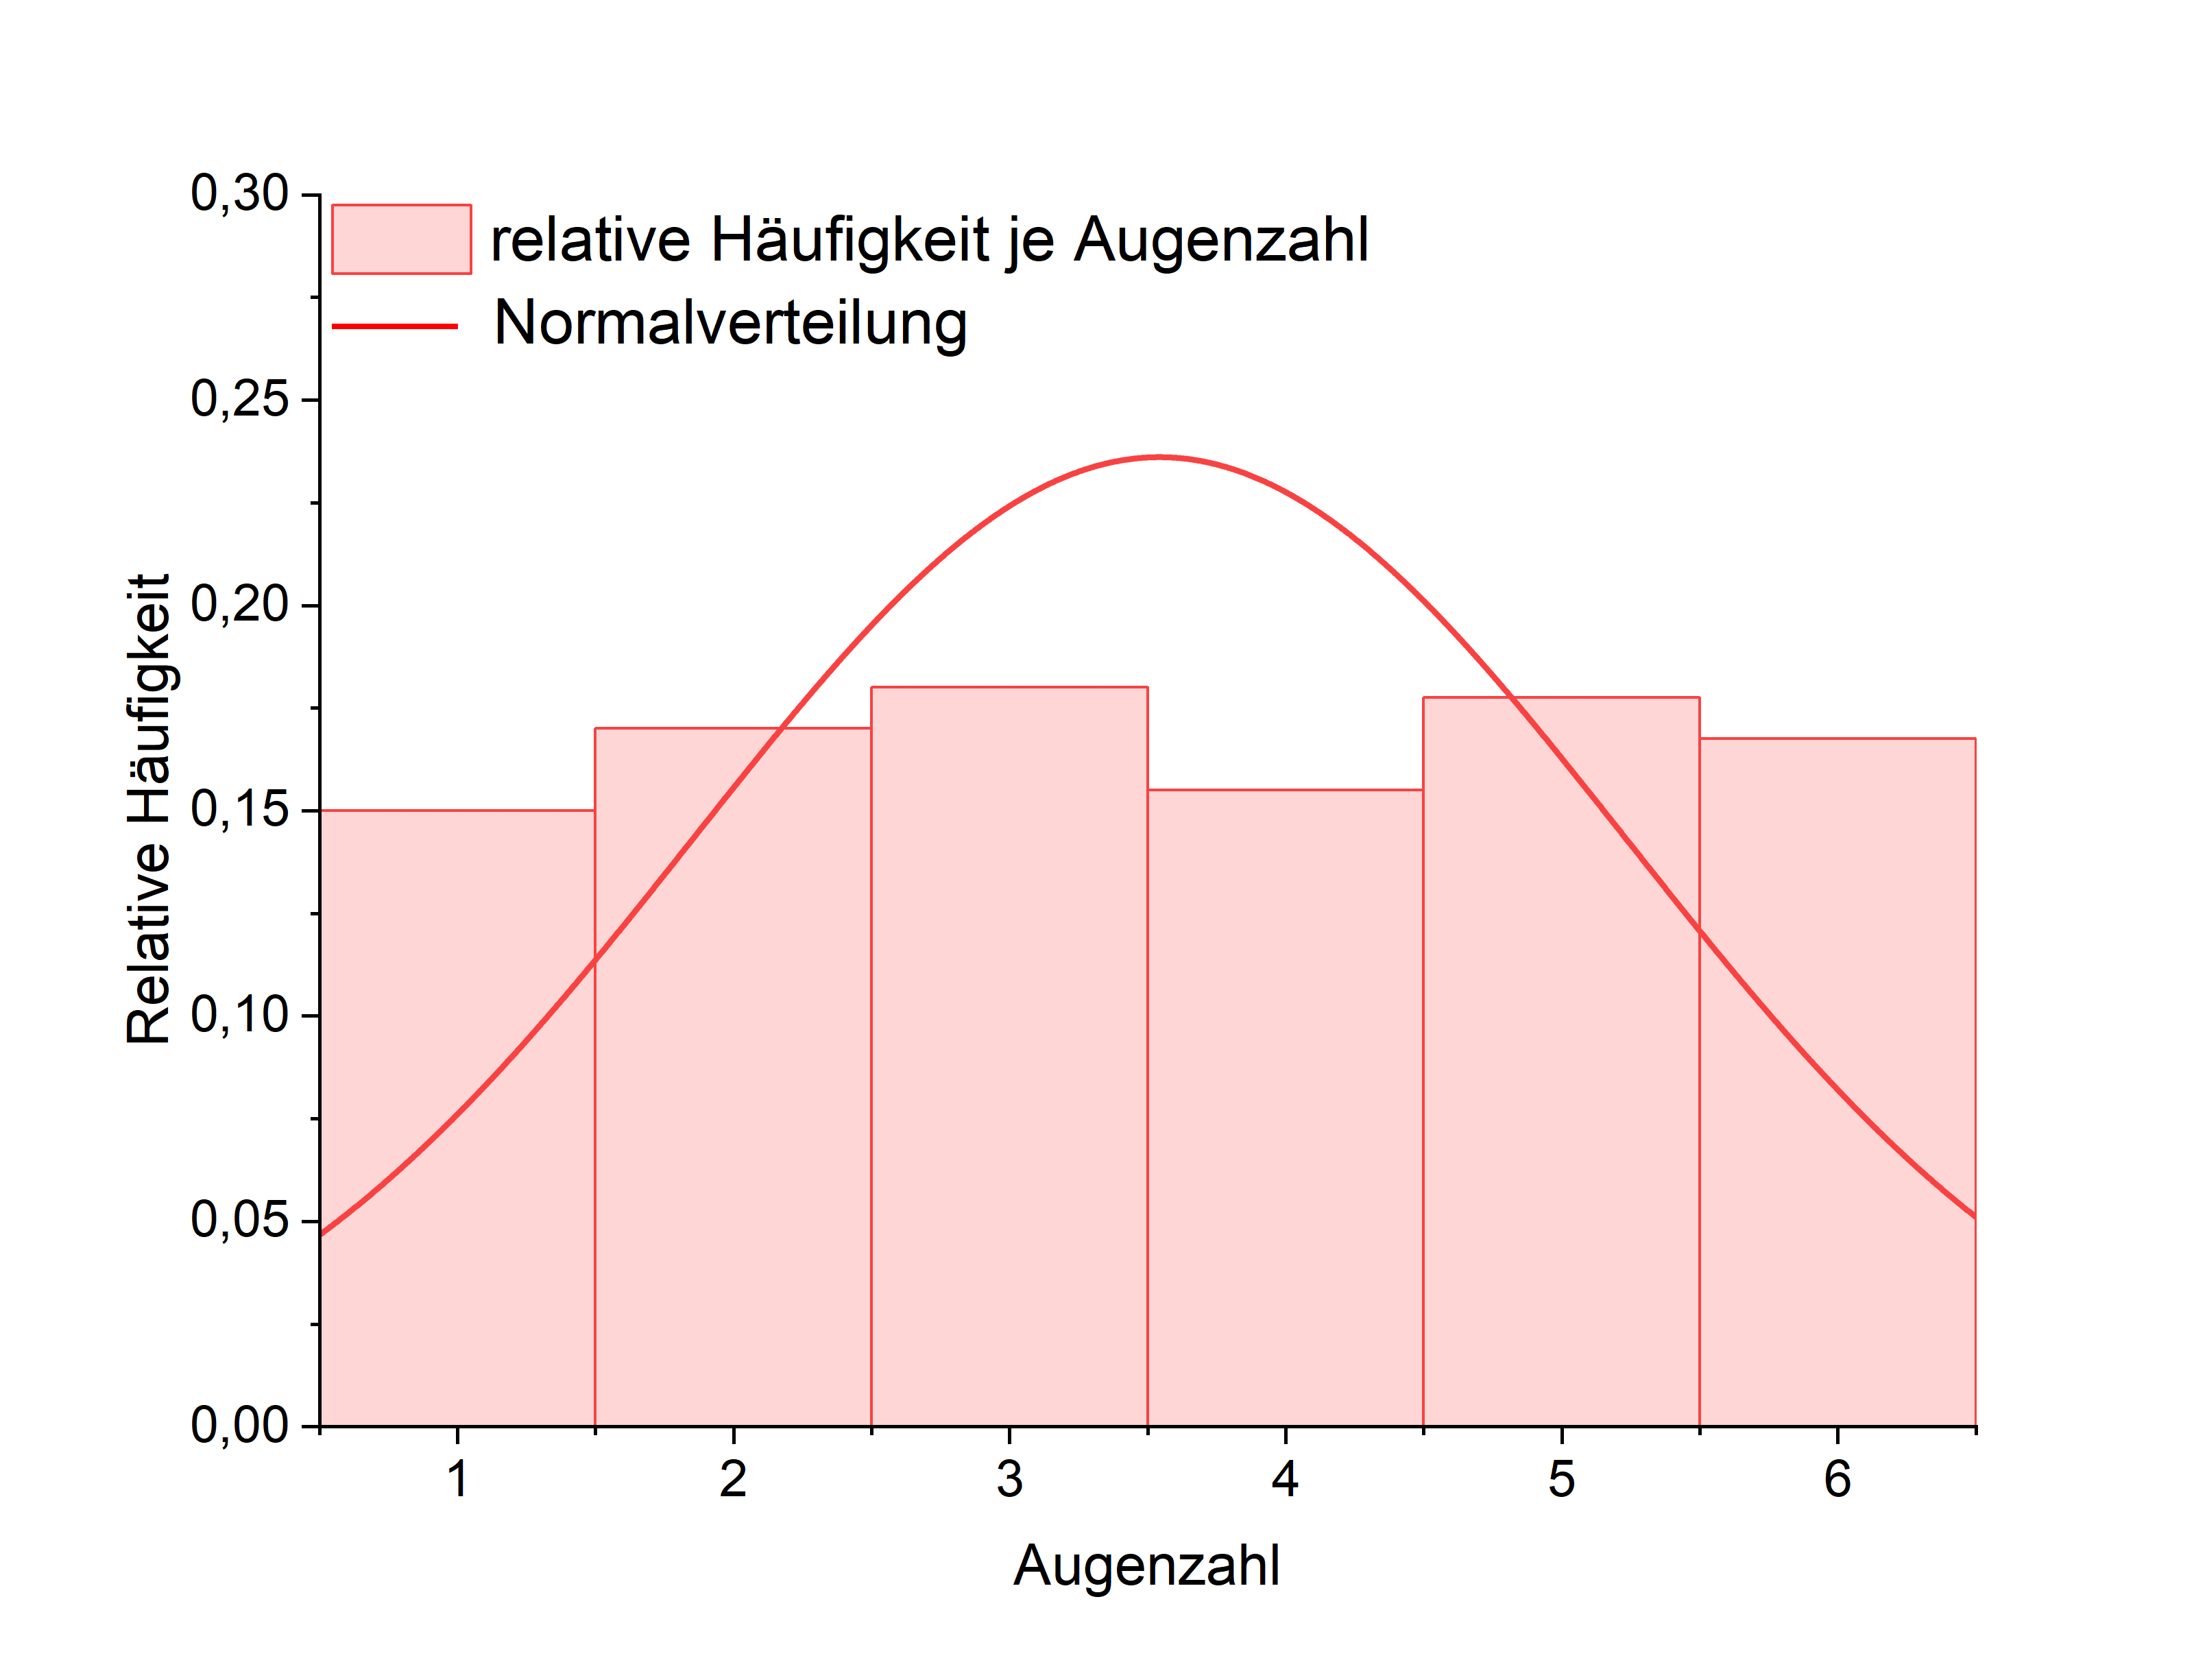
\includegraphics[width=\textwidth]{bilder/Diagramm1.png}        %// [ ] TODO: Diagramm Bild anpassen
    \caption{<>}                                                    %// [ ] TODO: Diagramm Bildunterschrift anpassen
\end{figure}

\section{Diskussion}
%//[ ] TODO: Diskussion
% Wie vergleicht sich meine Messung mit anderen Messungen/Theorien?
% Ist der Messwert sinnvoll? Stimmt die Größenordnung?
% Wo wurden Fehler gemacht? Was kann man verbessern?
% Gegebenenfalls rekursiv auswerten oder nachmessen!
% ursprüngliche Fragestellung diskutieren
% zB Standardabweichung diskutieren, berechnete Größen nennen

<>

\section{Anhang}
\subsection{Messprotokoll}
\label{Messprotokoll}


\begin{multicols}{3}

    \begin{table}[H]
        \centering
        \begin{tabular}{|c|c|}
            \hline
            & Zeit / $\mathrm{ms}$ \\
            \hline
            1 & 125.004 \\
            2 & 125.008 \\
            3 & 124.990 \\
            4 & 124.984 \\
            5 & 124.989 \\
            6 & 124.996 \\
            7 & 124.991 \\
            8 & 124.997 \\
            9 & 125.002 \\
            10 & 124.999 \\
            11 & 125.006 \\
            12 & 125.009 \\
            13 & 125.009 \\
            14 & 125.020 \\
            15 & 125.010 \\
            16 & 125.019 \\
            17 & 125.014 \\
            18 & 125.014 \\
            19 & 125.019 \\
            20 & 125.013 \\
            21 & 125.011 \\
            22 & 125.009 \\
            23 & 125.015 \\
            24 & 124.998 \\
            25 & 125.021 \\
            26 & 125.020 \\
            27 & 125.015 \\
            28 & 125.018 \\
            29 & 125.018 \\
            30 & 125.018 \\
            31 & 125.018 \\
            32 & 125.012 \\
            33 & 125.022 \\
            34 & 125.012 \\
            35 & 125.021 \\
            36 & 125.018 \\
            37 & 125.028 \\
            38 & 125.019 \\
            39 & 125.027 \\
            40 & 125.026 \\
            41 & 125.026 \\
            42 & 125.015 \\
            43 & 125.028 \\
            \hline
        \end{tabular}
    \end{table}
    \columnbreak
    \begin{table}[H]
        \centering
        \begin{tabular}{|c|c|}
            \hline
            44 & 125.019 \\
            45 & 125.020 \\
            46 & 125.012 \\
            47 & 125.023 \\
            48 & 125.041 \\
            49 & 125.042 \\
            50 & 125.032 \\
            51 & 125.021 \\
            52 & 125.028 \\
            53 & 125.023 \\
            54 & 125.037 \\
            55 & 125.036 \\
            56 & 125.026 \\
            57 & 125.020 \\
            58 & 125.031 \\
            59 & 125.023 \\
            60 & 125.029 \\
            61 & 125.032 \\
            62 & 125.028 \\
            63 & 125.036 \\
            64 & 125.029 \\
            65 & 125.031 \\
            66 & 125.027 \\
            67 & 125.034 \\
            68 & 125.029 \\
            69 & 125.036 \\
            70 & 125.031 \\
            71 & 125.047 \\
            72 & 125.033 \\
            73 & 125.038 \\
            74 & 125.039 \\
            75 & 125.032 \\
            76 & 125.037 \\
            77 & 125.035 \\
            78 & 125.029 \\
            79 & 125.036 \\
            80 & 125.029 \\
            81 & 125.030 \\
            82 & 125.032 \\
            83 & 125.036 \\
            84 & 125.026 \\
            85 & 125.035 \\
            86 & 125.052 \\
            87 & 125.052 \\
            \hline
        \end{tabular}
    \end{table}
    \columnbreak
    \begin{table}[H]
        \centering
        \begin{tabular}{|c|c|}
            \hline
            88 & 125.057 \\
            89 & 125.050 \\
            90 & 125.053 \\
            91 & 125.051 \\
            92 & 125.051 \\
            93 & 125.039 \\
            94 & 125.047 \\
            95 & 125.060 \\
            96 & 125.058 \\
            97 & 125.057 \\
            98 & 125.061 \\
            99 & 125.076 \\
            100 & 125.064 \\
            101 & 125.063 \\
            102 & 125.067 \\
            103 & 125.062 \\
            104 & 125.056 \\
            105* & 104.715 \\
            106 & 125.056 \\
            107 & 125.070 \\
            108 & 125.082 \\
            109 & 125.068 \\
            110 & 125.075 \\
            111 & 125.073 \\
            112 & 125.074 \\
            113 & 125.076 \\
            114 & 125.082 \\
            115 & 125.085 \\
            116 & 125.088 \\
            117 & 125.092 \\
            118 & 125.095 \\
            119 & 125.090 \\
            120 & 125.097 \\
            121 & 125.099 \\
            122 & 125.101 \\
            123 & 125.093 \\
            124 & 125.118 \\
            125 & 125.111 \\
            126 & 125.102 \\
            127 & 125.100 \\
            128 & 125.093 \\
            129 & 125.101 \\
            130 & 125.095 \\
            131 & 125.097 \\
            \hline
        \end{tabular}
    \end{table}
    \columnbreak
    \begin{table}[H]
        \centering
        \begin{tabular}{|c|c|}
            \hline
            132 & 125.100 \\
            133 & 125.094 \\
            134 & 125.104 \\
            135 & 125.098 \\
            136 & 125.104 \\
            137 & 125.105 \\
            138 & 125.097 \\
            139 & 125.105 \\
            140 & 125.099 \\
            141 & 125.098 \\
            142 & 125.111 \\
            143 & 125.108 \\
            144 & 125.112 \\
            145 & 125.121 \\
            146 & 125.120 \\
            147 & 125.114 \\
            148 & 125.117 \\
            149 & 125.123 \\
            150 & 125.126 \\
            151 & 125.124 \\
            152 & 125.134 \\
            153 & 125.138 \\
            154 & 125.131 \\
            155 & 125.140 \\
            156 & 125.128 \\
            157 & 125.126 \\
            158 & 125.135 \\
            159 & 125.136 \\
            160* & 106.664 \\
            161 & 125.148 \\
            162 & 125.162 \\
            163 & 125.161 \\
            164 & 125.148 \\
            165 & 125.156 \\
            166 & 125.148 \\
            167 & 125.143 \\
            168 & 125.150 \\
            169 & 125.148 \\
            170 & 125.175 \\
            171 & 125.182 \\
            172 & 125.171 \\
            173 & 125.163 \\
            174 & 125.152 \\
            175 & 125.166 \\
            \hline
        \end{tabular}
    \end{table}
    \columnbreak
    \begin{table}[H]
        \centering
        \begin{tabular}{|c|c|}
            \hline
            176 & 125.147 \\
            177 & 125.163 \\
            178 & 125.164 \\
            179 & 125.165 \\
            180 & 125.167 \\
            181 & 125.169 \\
            182 & 125.168 \\
            183 & 125.176 \\
            184 & 125.183 \\
            185 & 125.185 \\
            186 & 125.181 \\
            187 & 125.195 \\
            188 & 125.208 \\
            189 & 125.207 \\
            190 & 125.212 \\
            191 & 125.196 \\
            192 & 125.177 \\
            193 & 125.172 \\
            194 & 125.139 \\
            \hline
        \end{tabular}
        \caption{Messergebnisse}
    \end{table}
    
    \end{multicols}


\end{document}
